\documentclass{beamer}
\usepackage{graphicx}
%Information to be included in the title page:
\title{Sample title}
\author{Anonymous}
\institute{Overleaf}
\date{2021}

\begin{document}

\frame{\titlepage}

\begin{frame}
\frametitle{Background 1-2 min}

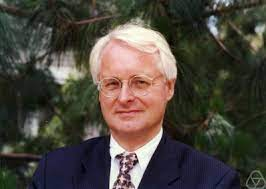
\includegraphics[scale = .5]{lenstra.jpeg}

\begin{itemize}
\item Hendrik Lenstra Jr. recieved his doctorate from the University of Amsterdam in 1977.

\item Discovered Elliptic Curve Factorization (ECM) in 1987.

\item ECM is third-fastest known factoring algorithm and the best algorithm for finding divisors not exceeding 50-60 digits.

\item The largest factor found using ECM has 83 digits.
\end{itemize}
\end{frame}

\begin{frame}
\frametitle{Preliminaries 2 mins} 
\begin{itemize}
\item Let $E$ be an elliptic curve over $\mathbb{Z}/N\mathbb{Z}$ of the form
$$
	y^2 = x^3 + ax + 1
$$
such that $4a^3 + 27 \in \left(\mathbb{Z}/N\mathbb{Z}\right)^*$. This forces non singularity and ensures $P = (0,1)$ is on the curve.

\item Definition 6.3.1 (Power Smooth). Let $B$ be a positive integer. If $n$ is a positive integer with prime factorization 
$$
    n = \prod p_i^{e_i},
$$
then $n$ is $B$-power smooth if $p_i^{e_i} \leq B$ for all $i$. 

\item Example $30 = 2\cdot 3\cdot 5$ is $B$ power smooth for $B \geq 5$, but $150 = 2\cdot 3 \cdot 5^2$ is not $5$-power smooth.
\end{itemize}
\end{frame}

\begin{frame}
\frametitle{Motivation 1-2 mins}
% Explain why p-1 not being B power smooth for a fixed B is a problem
\end{frame}

\begin{frame}
\frametitle{Elliptic Curve Factorization 2 mins}

\end{frame}

\begin{frame}
\frametitle{Analogy to Pollard p-1 1 min}

\end{frame}

\begin{frame}
\frametitle{Why it works 1-2 mins}

\end{frame}

\begin{frame}
\frametitle{Example by hand 2 mins}

\end{frame}

\begin{frame}
\frametitle{Implementation 2 mins}

\end{frame}

\begin{frame}
\frametitle{Run Time Analysis/Comparison 2 mins}

\end{frame}

\begin{frame}
\frametitle{Coded Example 2 mins}

\end{frame}

\begin{frame}
\frametitle{Animation 1 min}

\end{frame}

\end{document}